\documentclass[12pt,a4paper]{article}
\usepackage[utf8]{inputenc}
\usepackage[portuguese]{babel}
\usepackage{graphicx}
\usepackage{amsmath}
\usepackage{hyperref}

\title{Tópicos em Engenharia Computacional II\\Trabalho Prático 2024/2025}
\author{}
\date{}

\begin{document}

\maketitle

\tableofcontents
\newpage

\section{Introdução}

\section{Dados e Metodologia}

\section{Resultados}

\subsection{Deposição de Energia}

\subsection{Distribuição de Hits}

\subsection{Vértices Hadrónicos}

\subsection{Distribuição Temporal}

\subsection{Distribuição do Momento}

Nesta secção, é apresentada a análise da componente longitudinal do momento ($p_Z$) das partículas detetadas na simulação. A análise foca-se nos muões ($\mu^{\pm}$) e piões ($\pi^{\pm}$), e explora adicionalmente a distinção crucial entre piões primários (gerados na colisão inicial do feixe com o alvo) e secundários (produzidos em interações secundárias ou decaimentos).

De forma a garantir o rigor científico e evitar a duplicação estatística de contagens (uma vez que uma única partícula pode registar múltiplos \textit{hits} ao atravessar sucessivas camadas de detetores), os dados foram extraídos diretamente a nível de trajetória (\textit{track}) através do ramo \texttt{tracksData}. Como os histogramas são apresentados em escala logarítmica, foram considerados apenas valores positivos de $p_Z$.

\subsubsection{Comparação entre Muões e Piões}

A Figura~\ref{fig:momentum_muons_pions} apresenta os espectros de momento longitudinal $p_Z$ comparativos para muões e piões. Ambas as distribuições são apresentadas em escala logarítmica para permitir a visualização de ordens de grandeza muito distintas na estatística e gama de momentos.

\begin{figure}[htbp]
    \centering
    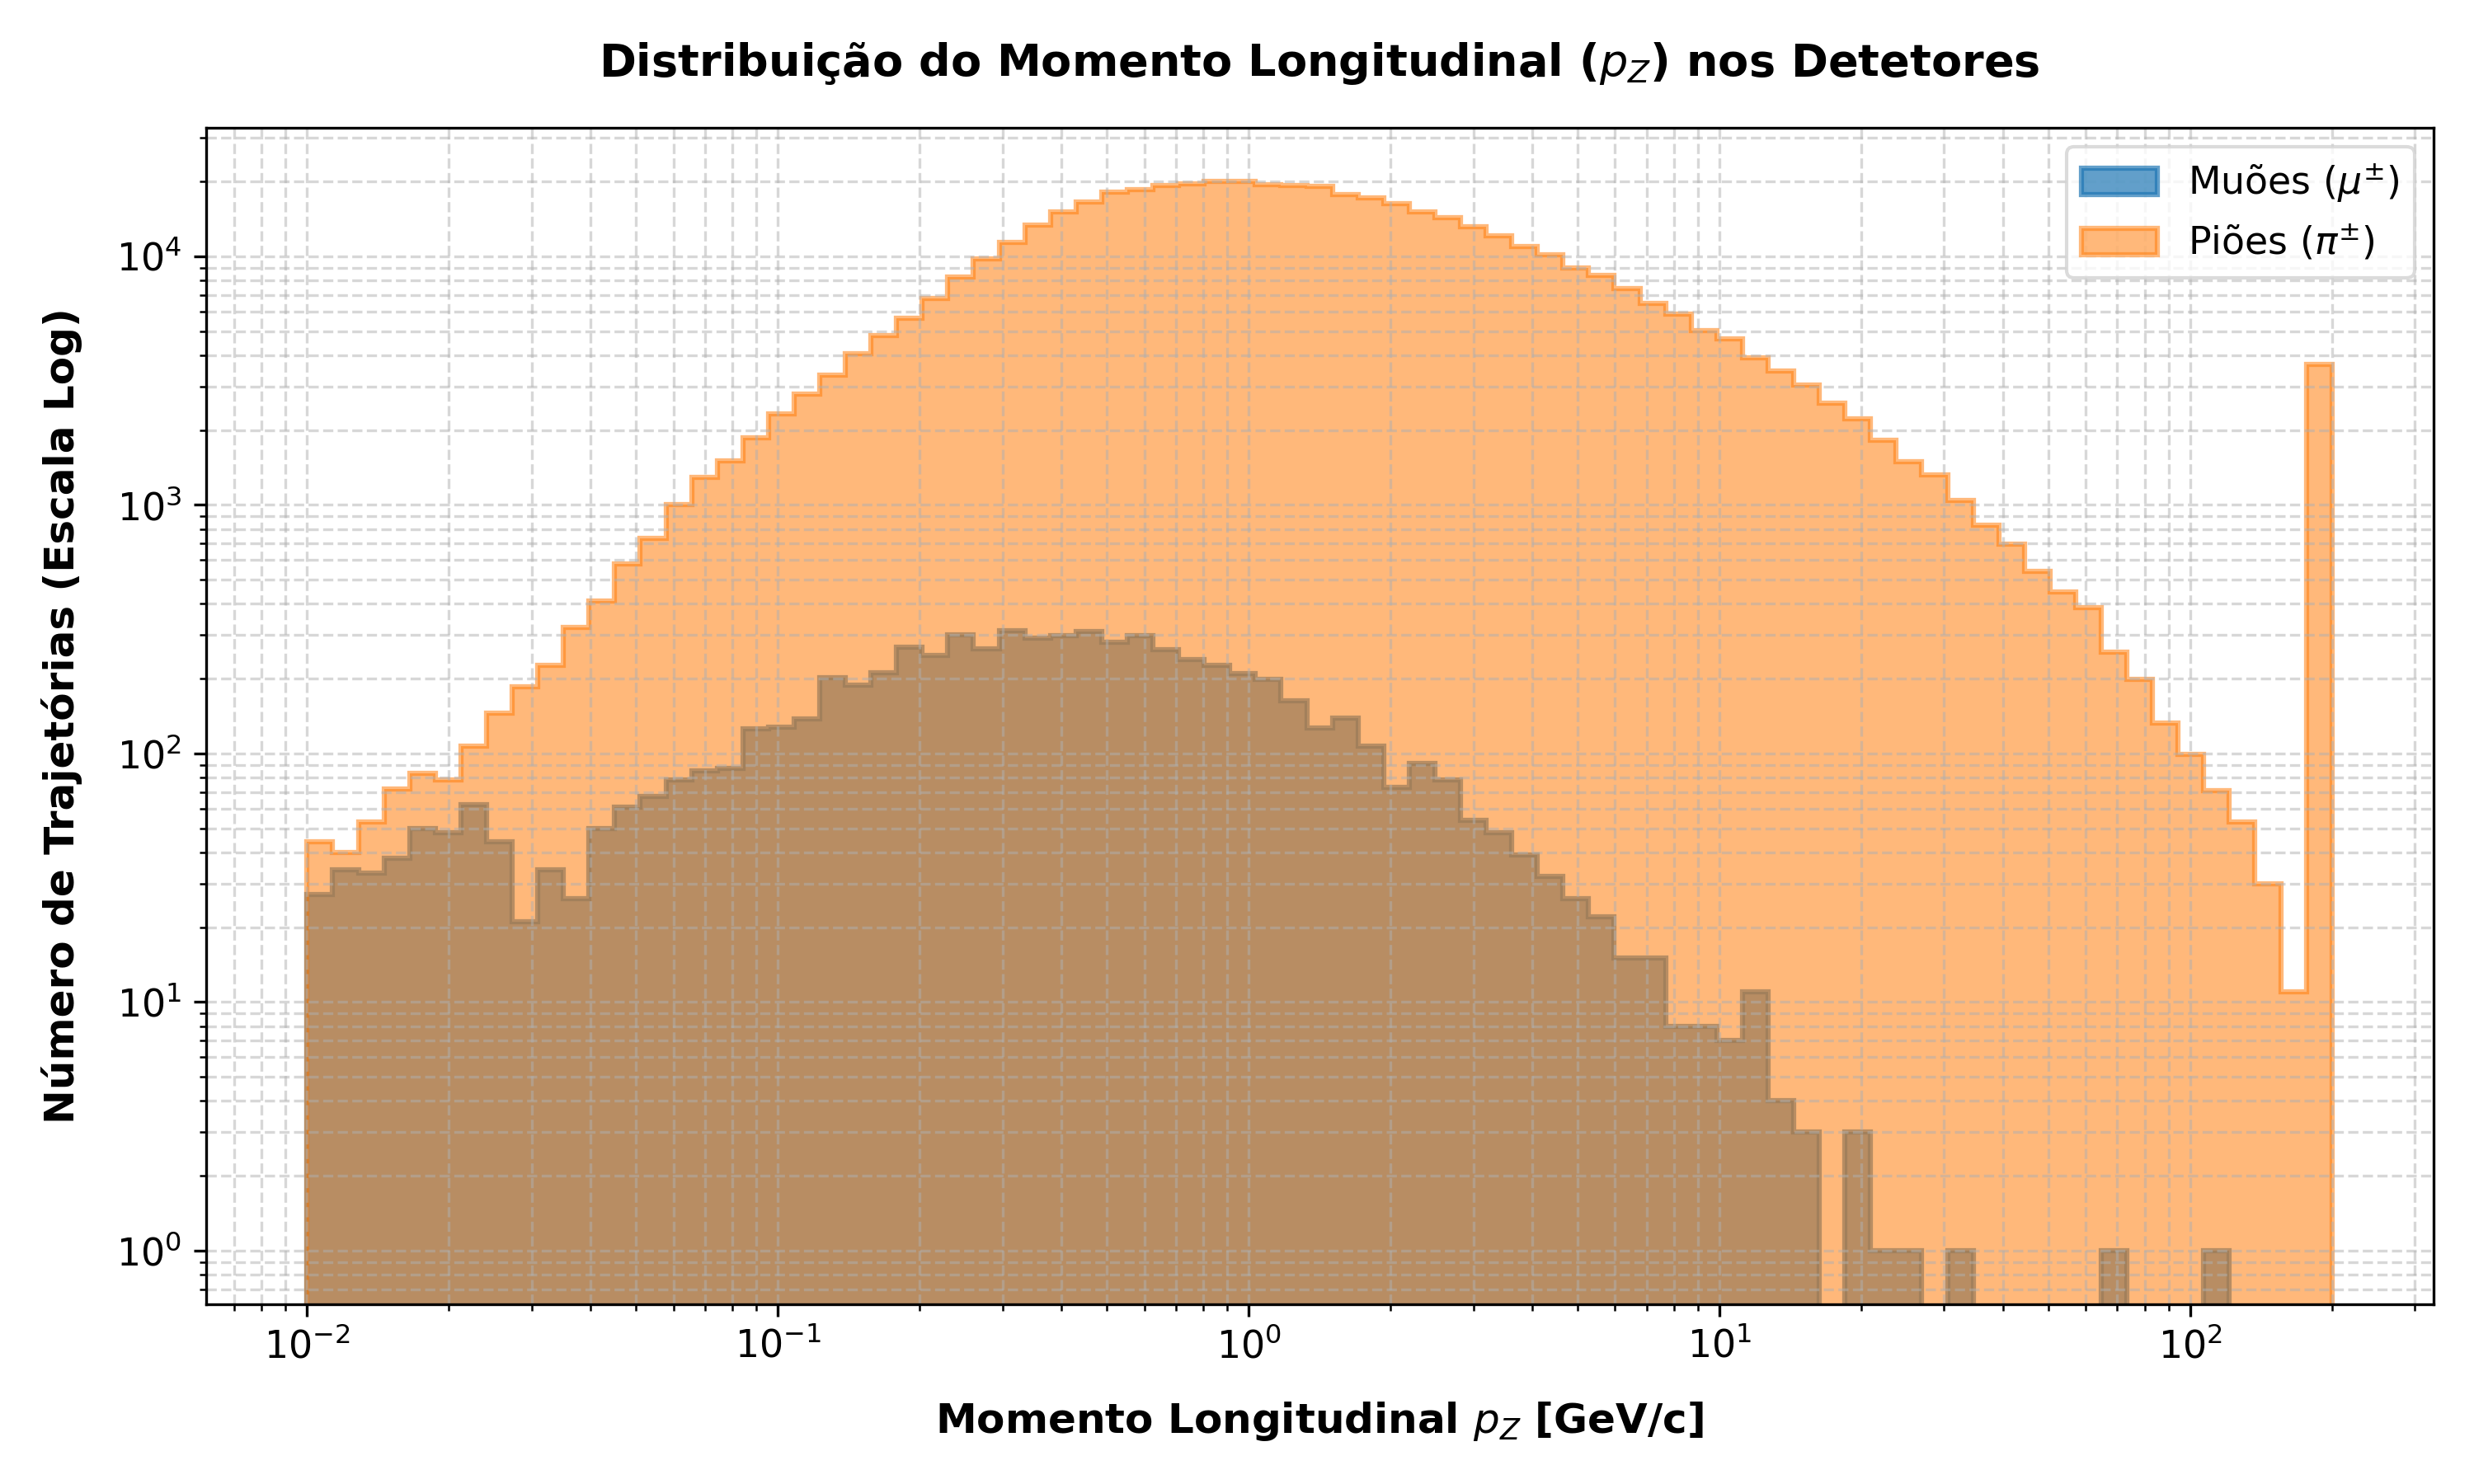
\includegraphics[width=0.85\textwidth]{../plots/momentum/momentum_muons_pions.png}
    \caption{Distribuição do momento longitudinal ($p_Z$) para muões ($\mu^{\pm}$) e piões ($\pi^{\pm}$).}
    \label{fig:momentum_muons_pions}
\end{figure}

Observa-se que os piões constituem a larga maioria das trajetórias produzidas na simulação, estendendo-se por uma vasta gama de momentos até cerca de $200$~GeV/c. Por outro lado, os muões apresentam um espectro muito mais concentrado em momentos baixos e intermédios: a maioria encontra-se abaixo de alguns GeV/c, embora exista uma cauda estatística rara para momentos superiores. Esta distinção é consistente com a natureza das partículas: os piões, sendo mesões que sofrem interação forte, são massivamente produzidos em colisões hadrónicas de alta energia, enquanto os muões são sobretudo resultantes de decaimentos ou processos eletromagnéticos de menor transferência de momento.

\subsubsection{Piões Primários vs. Secundários}

A comparação entre o momento dos piões primários e secundários é exibida na Figura~\ref{fig:momentum_pions_generation}.

\begin{figure}[htbp]
    \centering
    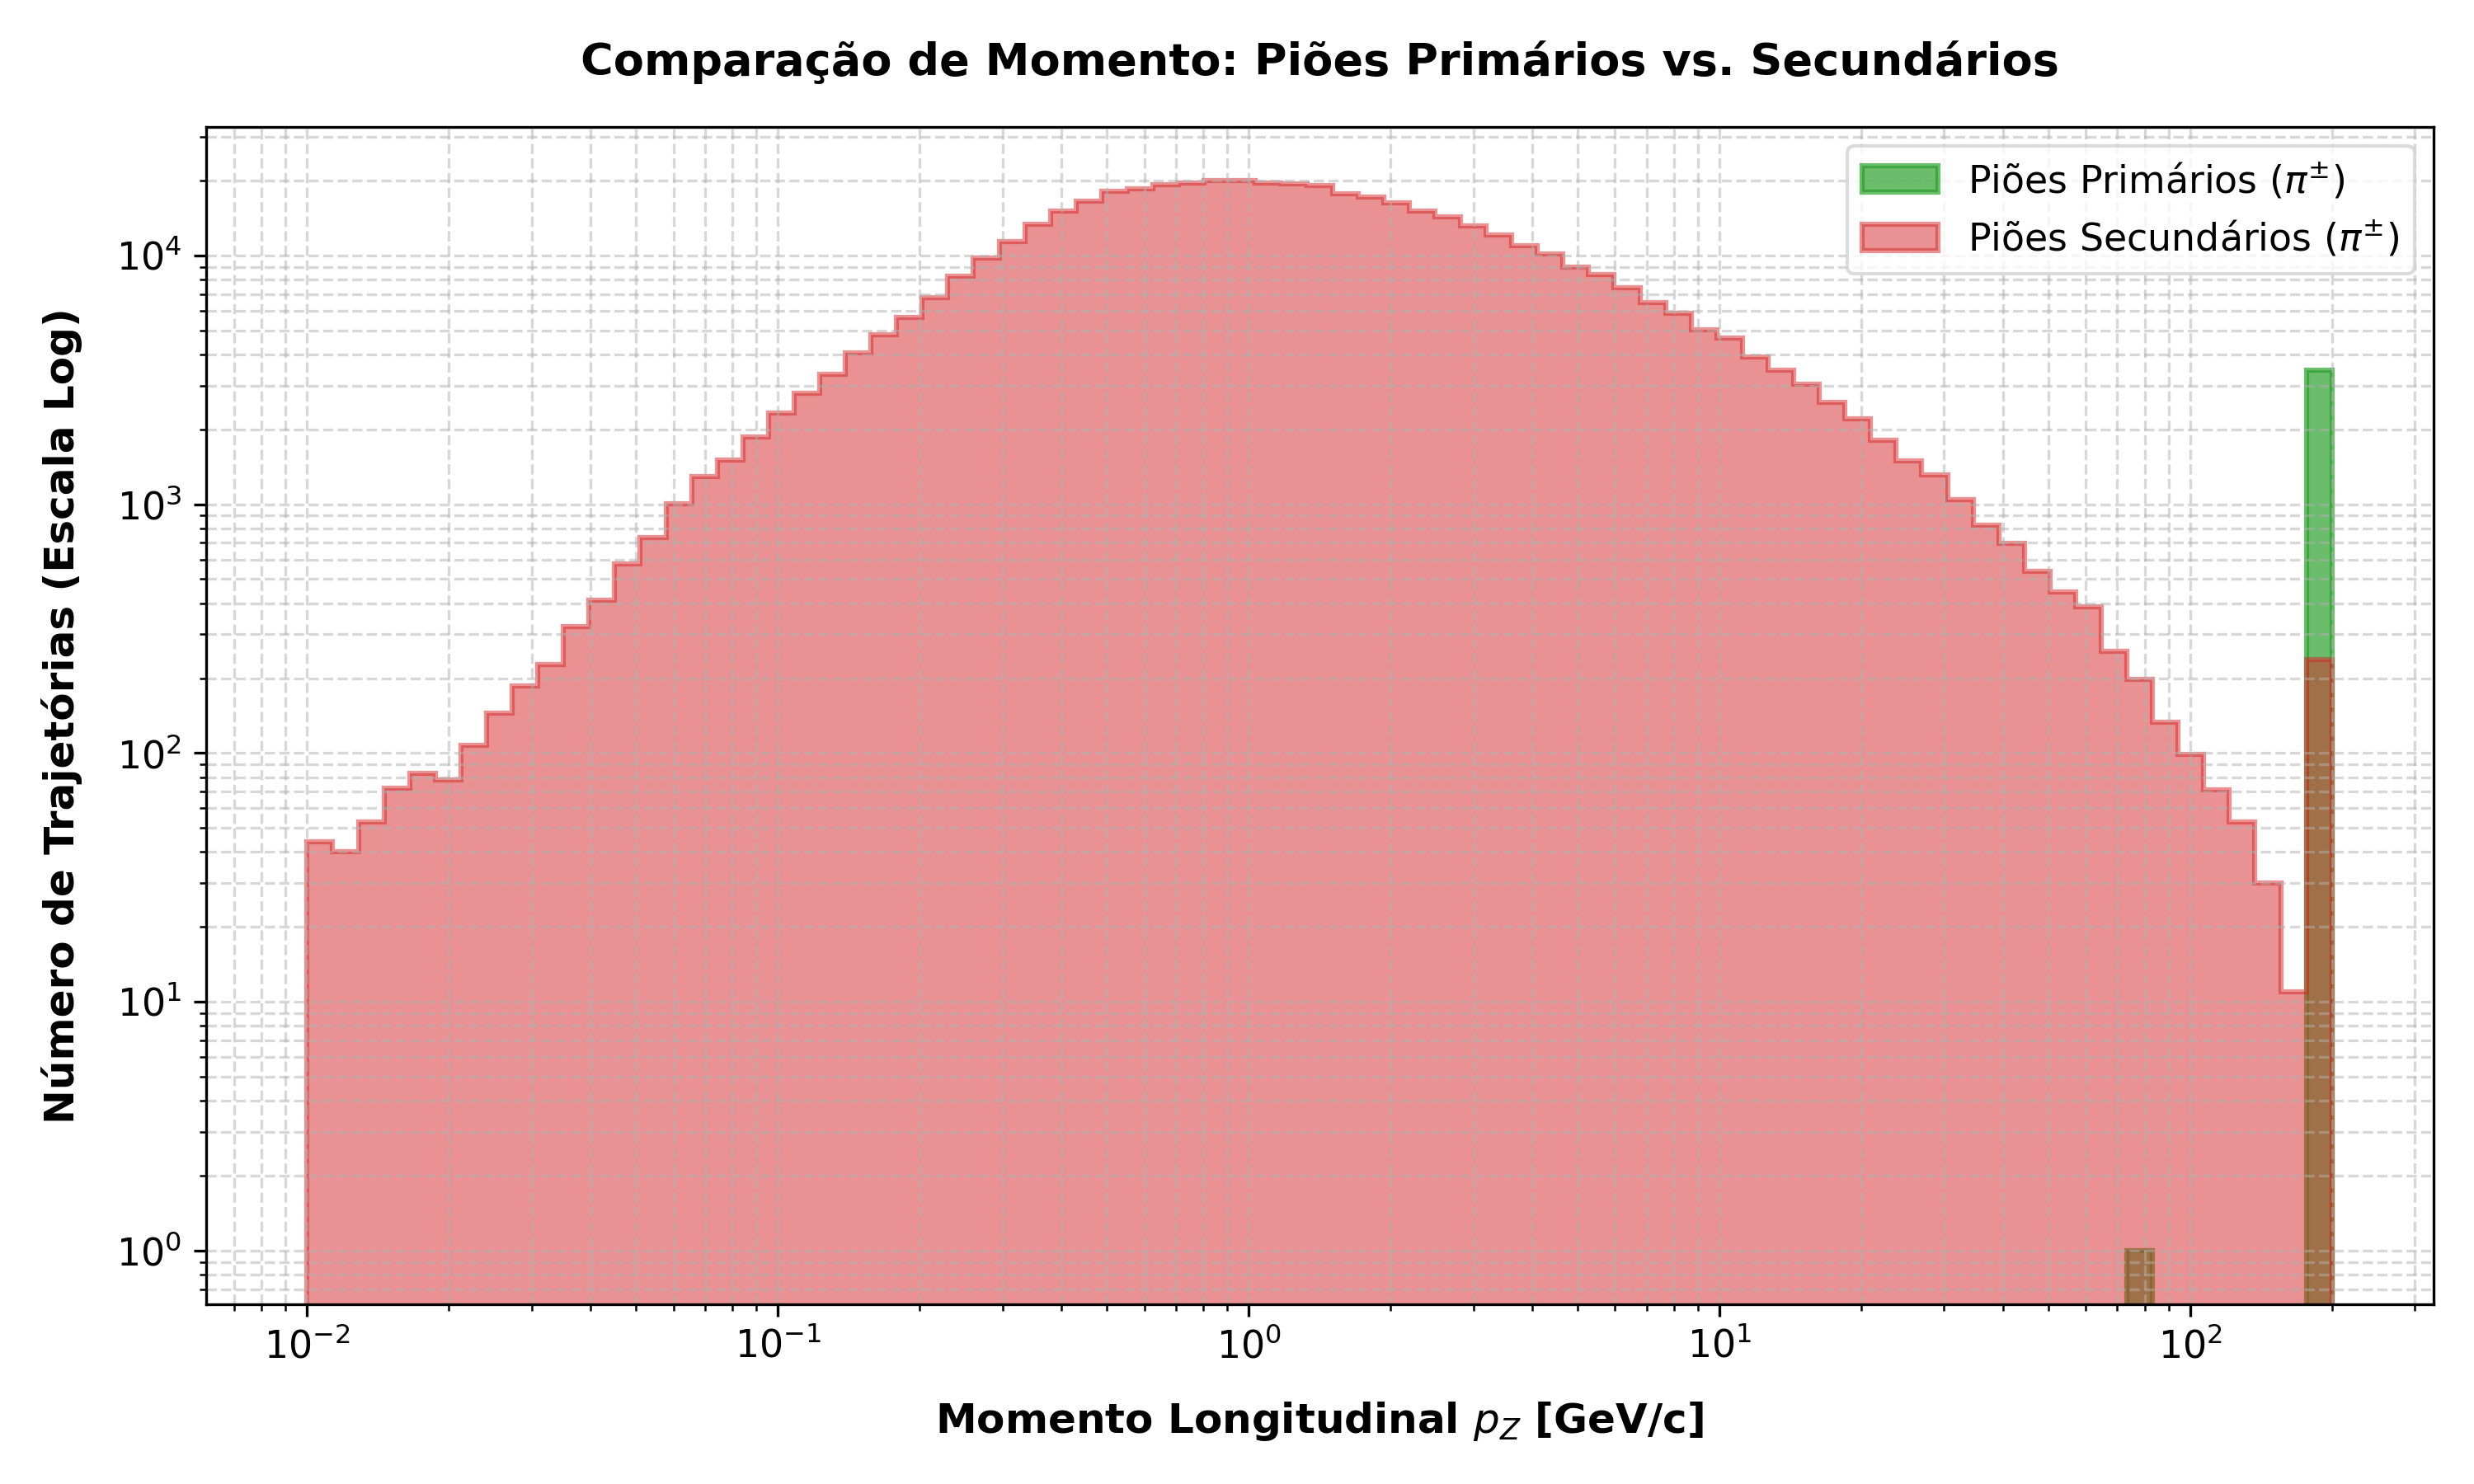
\includegraphics[width=0.85\textwidth]{../plots/momentum/momentum_pions_generation.png}
    \caption{Comparação da distribuição do momento longitudinal ($p_Z$) para piões primários (geração direta) e secundários.}
    \label{fig:momentum_pions_generation}
\end{figure}

A análise revela uma distinção física muito nítida entre as duas categorias:
\begin{itemize}
    \item \textbf{Piões Primários:} Apresentam um espectro de momento substancialmente mais energético, herdando uma fração significativa do momento do feixe inicial. O seu perfil estende-se até ao limite cinemático superior.
    \item \textbf{Piões Secundários:} São muito mais numerosos na simulação, mas o seu momento longitudinal está fortemente concentrado em energias baixas, com a grande maioria abaixo de algumas dezenas de GeV/c e uma cauda de alta energia menos populada. Isto deve-se ao facto de serem gerados em colisões hadrónicas secundárias em cascata (por exemplo, interações inelásticas do tipo \textit{pi-Inelastic} no interior ou na vizinhança do alvo), onde a energia do feixe é progressivamente partilhada por múltiplas partículas filhas de menor momento.
\end{itemize}

\section{Conclusão}

\end{document}
